\documentclass[sigconf,anonymous,review]{acmart}

\usepackage{amsfonts,amsmath,amsthm,booktabs,graphicx,mathtools,xcolor}
\usepackage{hyperref}

\newtheorem{theorem}{Theorem}[section]
\newtheorem{lemma}[theorem]{Lemma}
\newtheorem{assumption}[theorem]{Assumption}
\newtheorem{remark}[theorem]{Remark}

% comment 
\newcommand{\xg}[1]{\textcolor{red}{[Xi: #1]}}
\newcommand{\david}[1]{\textcolor{red}{[David: #1]}}

\AtBeginDocument{%
  \providecommand\BibTeX{{Bib\TeX}}}

\begin{document}

\title{A/B Testing with Exposure-Dependent User Response}

\begin{abstract}
Standard A/B-test summaries target a single average effect and therefore obscure how user response changes with repeated exposure to a new product surface. In many applications, it is important to report this dynamic in addition to the average treatment effect: an intervention may initially slow users down and only later improve efficiency, or may exhibit the opposite pattern as novelty wears off. Estimating how response changes over repeated use requires care when users contribute different numbers of exposures within the experiment window. A naive exposure-by-exposure average is confounded by changing user composition.

We study a simple additive model for the conditional mean surface,
\[
\mathbb{E}[Y_{ij}\mid T_i=t]=a_0(t)+b_0(j),
\]
\xg{Should I remove the precise model formulation here and replace it with: ``We study an additive model in which average outcomes depend on both a user's total number of exposures and the current exposure index.''}
where $Y_{ij}$ is the outcome at exposure $j$ for user $i$, $T_i$ is the total number of exposures observed for user $i$, $a_0(t)$ captures differences across users with different total numbers of exposures, and $b_0(j)$ captures how mean response changes with exposure. We estimate $(a_0,b_0)$ by least squares under the normalization $b_0(1)=0$. We show that the estimator is conditionally unbiased for $b_0$, consistent, and asymptotically normal when the exposure horizon is fixed. We further establish first-order validity of the standard user-level bootstrap for inference and show that the naive column-mean estimator generally targets a different limit and can therefore have asymptotically vanishing coverage for the quantity of interest.
\end{abstract}

\begin{CCSXML}
<ccs2012>
   <concept>
       <concept_id>10002944.10011123.10011131</concept_id>
       <concept_desc>General and reference~Experimentation</concept_desc>
       <concept_significance>500</concept_significance>
   </concept>
</ccs2012>
\end{CCSXML}

\ccsdesc[500]{General and reference~Experimentation}

\keywords{A/B testing, exposure-response curve, semiparametric estimation, clustered bootstrap}

\maketitle

\section{Introduction}

A product change can affect users differently across repeated exposures. An intervention may attenuate as initial novelty fades, or it may strengthen as users become familiar with a new interface. In such settings, a single average treatment-effect summary can be difficult to interpret and may be inadequate for product decisions. Standard experimentation practice often emphasizes overall treatment effects and other low-dimensional summaries \cite{Kohavi2008}. Recent work on long-term online experiments has emphasized that such summaries can miss novelty, primacy, and delayed treatment effects \cite{Hohnhold2015,Dmitriev2016,Sadeghi2022}. These papers motivate moving beyond one-number summaries, but their focus is long-term or calendar-time treatment effects. Our object is different: we index response by the exposure count itself and address the composition change induced by the fact that later exposures are observed only for users with longer realized histories.

To motivate the problem, consider an online experiment on a social-networking app. The product team launches a redesigned direct-message reply composer that slightly reduces friction through faster keyboard focus, fewer taps, and quicker attachment access. Heavy and light users may differ substantially in their baseline messaging speed, yet the shape of ``getting used to'' the new interface may still be similar across user types.

Suppose the team runs an A/B test for two weeks and is interested not only in whether the redesign improves average performance, but also in how user response evolves across repeated uses. Let $T_i\in\{1,\dots,B\}$ denote the number of direct messages sent by user $i$ during the experiment window, and let $Y_{ij}\in\mathbb{R}$ denote the outcome for the $j$th exposure, for $j\in[T_i]:=\{1,\dots,T_i\}$. For concreteness, one may take $Y_{ij}$ to be the time spent composing the $j$th message.

A standard summary is the average within-user outcome,
\[
\hat\theta_{\mathrm{avg}}
=
\frac{1}{n}\sum_{i=1}^n \frac{1}{T_i}\sum_{j=1}^{T_i} Y_{ij},
\]
together with a usual $z$-interval based on the $n$ user-level averages. This is often reasonable for a one-number summary, but it does not isolate how response changes with exposure. If the redesign initially slows users down and only later improves efficiency, then $\hat\theta_{\mathrm{avg}}$ conflates these effects.

A natural alternative is the exposure-specific average
\[
\left\{
\frac{1}{|\{i:T_i\ge j\}|}
\sum_{i:T_i\ge j} Y_{ij}
\right\}_{j=1}^B.
\]
This estimator is generally biased for the exposure profile of interest because the set $\{i:T_i\ge j\}$ changes with $j$. Later exposures are observed only for users who remain active long enough to reach them, so the estimate increasingly reflects the composition of heavier users.

At the other extreme, one may estimate the full triangular array of cell means,
\[
\left\{
\frac{1}{|\{i:T_i=t\}|}
\sum_{i:T_i=t} Y_{ij}
\right\}_{1\le j\le t\le B}.
\]
This removes the composition problem but introduces $\frac{B(B+1)}{2}$ mean parameters, which can lead to substantial variance.

These observations suggest a bias--variance tradeoff. We would like a model that adjusts for systematic differences across users with different total exposure counts, while avoiding a fully saturated cell-mean surface. Our proposal is a simple additive conditional-mean model on the triangular domain. It yields an exposure-response curve that is interpretable, easy to estimate, and amenable to bootstrap inference.

Methodologically, our proposal is related to classical repeated-measures analysis. Random-effects models and generalized estimating equations provide general tools for longitudinal outcomes \cite{LairdWare1982,LiangZeger1986}. Our focus is narrower: we exploit the triangular observation structure induced by a finite exposure window and target a parsimonious additive conditional-mean surface indexed by total exposure count and exposure index. This yields an exposure-response estimand tailored to online experimentation and directly addresses the composition bias that accumulates at later exposures.

For clarity, we formulate the method for a single arm. In a two-arm A/B test, one may fit the model separately in each arm and compare the resulting response curves, or apply the same construction to arm-specific contrasts.

\section{Setup and Estimand}

Fix a maximum exposure horizon $B\in\mathbb{N}$. For each user $i=1,\dots,n$, we observe a total number of exposures $T_i\in\{1,\dots,B\}$ and outcomes $(Y_{i1},\dots,Y_{iT_i})$. Define the user record
\[
Z_i := (T_i, Y_{i1},\dots,Y_{iT_i}).
\]
We assume throughout that $Z_1,\dots,Z_n$ are i.i.d. across users; within-user dependence in $(Y_{ij})_{j\le T_i}$ is unrestricted.

Let the triangular index set be
\[
\mathcal{D}:=\{(t,j):1\le j\le t\le B\}.
\]




We assume that there exist functions $a_0:\{1,\dots,B\}\to\mathbb{R}$ and $b_0:\{1,\dots,B\}\to\mathbb{R}$ such that
\begin{equation}
\mathbb{E}[Y_{ij}\mid T_i=t]=a_0(t)+b_0(j),
\qquad (t,j)\in\mathcal{D},
\label{eq:model}
\end{equation}
with the normalization
\begin{equation}
b_0(1)=0.
\label{eq:norm}
\end{equation}
The function $a_0(t)$ captures systematic differences across users who accumulate different total numbers of exposures within the experiment window, while $b_0(j)$ captures the common exposure profile. We refer to $\{b_0(j)\}_{j=1}^B$ as the \emph{response curve by exposure}. Under \eqref{eq:norm}, $b_0(j)$ is interpretable as the mean response at exposure $j$ relative to exposure $1$, after adjusting for composition through $a_0$.

\begin{figure}[t]
  \centering
  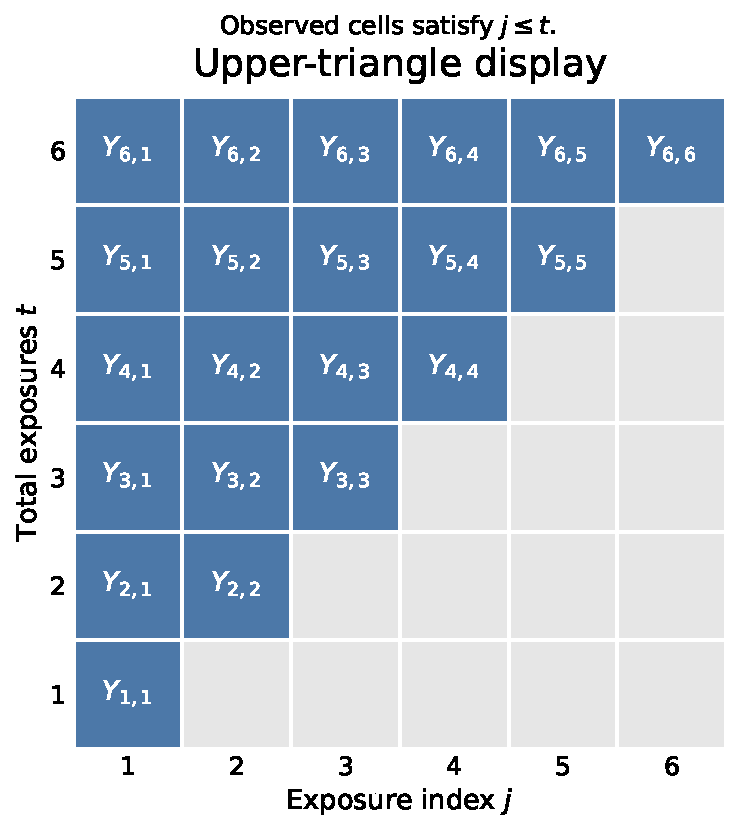
\includegraphics[width=0.78\linewidth]{figures/upper_triangular_layout_preview.pdf}
  \caption{Upper-triangular display of the observed data layout. A cell $(t,j)$ is observed only when $1 \le j \le t \le B$. Under the additive model, the conditional mean at each observed cell satisfies $\mathbb{E}[Y_{ij}\mid T_i=t]=a_0(t)+b_0(j)$.}
  \Description{An upper-triangular grid indexed by total exposures t and exposure index j. Cells with j less than or equal to t are observed and labeled Y_{t,j}; cells with j greater than t are unobserved.}
  \label{fig:triangular-layout}
\end{figure}

Define the regression error
\[
\varepsilon_{ij}:=Y_{ij}-a_0(T_i)-b_0(j).
\]
Then \eqref{eq:model} implies
\begin{equation}
\mathbb{E}[\varepsilon_{ij}\mid T_i]=0
\qquad\text{for all } j\le T_i.
\label{eq:meanzero}
\end{equation}

\xg{Explicitely state the estimand.}

\section{Method}

The additive model \eqref{eq:model} reduces the $\frac{B(B+1)}{2}$ unrestricted cell means on the triangular domain to $2B-1$ free parameters. This is the regularization that links the full cell-mean surface to a single exposure curve shifted by a length-specific intercept. It is a strong assumption, but it directly targets the bias--variance tradeoff described in the introduction.

Let
\[
\theta := \big(a(1),\dots,a(B),\,b(2),\dots,b(B)\big)^\top\in\mathbb{R}^{2B-1},
\]
where $b(1)\equiv 0$ is fixed. For each observed cell $(i,j)$ with $1\le j\le T_i$, define $x_{ij}\in\mathbb{R}^{2B-1}$ by placing a $1$ in the coordinate corresponding to $a(T_i)$, a $1$ in the coordinate corresponding to $b(j)$ when $j\ge 2$, and $0$ elsewhere. Then
\[
x_{ij}^\top\theta = a(T_i)+b(j).
\]

We estimate $\theta$ by least squares:
\begin{equation}
\hat\theta
:=
\arg\min_{\theta\in\mathbb{R}^{2B-1}}
\sum_{i=1}^n \sum_{j=1}^{T_i} \big(Y_{ij}-x_{ij}^\top\theta\big)^2.
\label{eq:ols}
\end{equation}
Write $\hat b(j)$ for the implied estimate of $b_0(j)$, with $\hat b(1)=0$.

For comparison, we also consider the naive column-mean estimator,
\[
\hat b_{\mathrm{naive}}(j)
=
\frac{1}{|\{i:T_i\ge j\}|}\sum_{i:T_i\ge j} Y_{ij}
-
\frac{1}{n}\sum_{i=1}^n Y_{i1},
\qquad j=1,\dots,B,
\]
with $\hat b_{\mathrm{naive}}(1)=0$. This estimator ignores the change in user composition across exposure indices.

\section{Identification and Finite-Sample Unbiasedness}

\begin{lemma}[Identification under $b_0(1)=0$]
\label{lem:ident}
Assume $\mathbb{P}(T_i=t)>0$ for all $t\in\{1,\dots,B\}$ and $\mathbb{P}(T_i\ge j)>0$ for all $j\in\{2,\dots,B\}$. If two pairs $(a,b)$ and $(a',b')$ satisfy
\[
a(t)+b(j)=a'(t)+b'(j)
\quad\text{for all } (t,j)\in\mathcal{D},
\qquad b(1)=b'(1)=0,
\]
then $a(t)=a'(t)$ for all $t$ and $b(j)=b'(j)$ for all $j$.
\end{lemma}

\xg{Mention how positivity violation can and should be addressed by coarsening the exposure bins.}

\begin{proof}
Fix $t\in\{1,\dots,B\}$. Evaluating the equality at $j=1$ gives
\[
a(t)+b(1)=a'(t)+b'(1),
\]
hence $a(t)=a'(t)$ because $b(1)=b'(1)=0$. Substituting back yields $b(j)=b'(j)$ for all $j\le t$. Since $\mathbb{P}(T_i\ge j)>0$ for each $j$, every exposure index appears in the triangular domain, so $b=b'$ on $\{1,\dots,B\}$.
\end{proof}

\begin{lemma}[Conditional unbiasedness of $\hat b$]
\label{lem:unbiased}
Assume \eqref{eq:model} and \eqref{eq:meanzero}. Let $X$ be the stacked design matrix whose rows are the vectors $x_{ij}^\top$ over all observed cells $(i,j)$ with $j\le T_i$. Suppose $X$ has full column rank. Then
\[
\mathbb{E}[\hat\theta\mid X]=\theta_0,
\qquad\text{and hence}\qquad
\mathbb{E}[\hat b(j)\mid X]=b_0(j)\quad\text{for all } j\ge 2.
\]
\end{lemma}

\begin{proof}
Stack the observed outcomes into a vector $Y$ and write
\[
Y=X\theta_0+\varepsilon,
\]
where $\varepsilon$ stacks the errors $\varepsilon_{ij}$. The least-squares estimator is
\[
\hat\theta=(X^\top X)^{-1}X^\top Y
=
\theta_0+(X^\top X)^{-1}X^\top\varepsilon.
\]
By \eqref{eq:meanzero}, $\mathbb{E}[\varepsilon\mid X]=0$, and therefore
\[
\mathbb{E}[\hat\theta\mid X]=\theta_0.
\]
The claim for $\hat b(j)$ follows by coordinate projection.
\end{proof}

\section{Large-Sample Validity of the Point Estimator}

\begin{assumption}[Regularity conditions for fixed $B$]
\label{ass:reg}
The following conditions hold.
\begin{enumerate}
\item $Z_1,\dots,Z_n$ are i.i.d.
\item $T_i\le B$ almost surely, with fixed $B$.
\item $\mathbb{E}\!\left[\sum_{j=1}^{T_i} Y_{ij}^2\right]<\infty$.
\item The matrix
\[
Q:=\mathbb{E}\!\left[\sum_{j=1}^{T_i} x_{ij}x_{ij}^\top\right]
\]
is positive definite.
\item The conditional-mean model \eqref{eq:model} holds.
\end{enumerate}
\end{assumption}

Define
\[
Q_i:=\sum_{j=1}^{T_i} x_{ij}x_{ij}^\top,
\qquad
q_i:=\sum_{j=1}^{T_i} x_{ij}Y_{ij},
\]
and the sample averages
\[
Q_n:=\frac{1}{n}\sum_{i=1}^n Q_i,
\qquad
q_n:=\frac{1}{n}\sum_{i=1}^n q_i.
\]
Whenever $Q_n$ is invertible, the estimator satisfies $\hat\theta=Q_n^{-1}q_n$.

\xg{The abuse of notation in $Q_i$ and $Q_n$ should be avoided. Try something like $\tilde Q$ instead.}

\begin{theorem}[Consistency and asymptotic normality]
\label{thm:clt}
Under Assumption~\ref{ass:reg},
\begin{enumerate}
\item $\hat\theta\xrightarrow{p}\theta_0$, and therefore $\hat b(j)\xrightarrow{p} b_0(j)$ for each fixed $j\ge 2$.
\item Let
\[
\psi_i:=\sum_{j=1}^{T_i} x_{ij}\varepsilon_{ij},
\qquad
\Omega:=\mathrm{Var}(\psi_i).
\]
Then
\[
\sqrt{n}(\hat\theta-\theta_0)
\Rightarrow
N\!\bigl(0,Q^{-1}\Omega Q^{-1}\bigr).
\]
Consequently, for each fixed $j\ge 2$,
\[
\sqrt{n}\bigl(\hat b(j)-b_0(j)\bigr)\Rightarrow N(0,v_j),
\]
where $v_j$ is the diagonal entry of $Q^{-1}\Omega Q^{-1}$ corresponding to the coordinate $b(j)$.
\end{enumerate}
\end{theorem}

\begin{proof}
By the law of large numbers applied to i.i.d.\ users, $Q_n\to_p Q$ and $q_n\to_p q:=\mathbb{E}[q_i]$. Under \eqref{eq:model} and \eqref{eq:meanzero},
\[
Y_{ij}=x_{ij}^\top\theta_0+\varepsilon_{ij}
\quad\text{with}\quad
\mathbb{E}[\varepsilon_{ij}\mid T_i]=0.
\]
Hence
\[
q
=
\mathbb{E}\!\left[\sum_{j=1}^{T_i} x_{ij}(x_{ij}^\top\theta_0+\varepsilon_{ij})\right]
=
Q\theta_0.
\]
Because $Q$ is invertible, $Q_n$ is invertible with probability tending to one, and
\[
\hat\theta
=
Q_n^{-1}q_n
\to_p
Q^{-1}(Q\theta_0)
=
\theta_0.
\]
This proves consistency.

For asymptotic normality, observe that
\[
Q_n(\hat\theta-\theta_0)
=
q_n-Q_n\theta_0
=
\frac{1}{n}\sum_{i=1}^n \sum_{j=1}^{T_i} x_{ij}\varepsilon_{ij}
=
\frac{1}{n}\sum_{i=1}^n \psi_i.
\]
Therefore,
\[
\sqrt{n}(\hat\theta-\theta_0)
=
Q_n^{-1}
\left(
\frac{1}{\sqrt{n}}\sum_{i=1}^n \psi_i
\right).
\]
The vectors $\psi_i$ are i.i.d.\ mean zero with finite covariance $\Omega$, so the multivariate central limit theorem yields
\[
\frac{1}{\sqrt{n}}\sum_{i=1}^n \psi_i
\Rightarrow
N(0,\Omega).
\]
Since $Q_n^{-1}\to_p Q^{-1}$, Slutsky's theorem gives the stated limit. The univariate result for $\hat b(j)$ follows by projection. See, for example, \cite[Chapters~5--6]{vdV1998}.
\end{proof}

\section{Bootstrap Validity for Our Method}

We use the standard nonparametric bootstrap at the user level: draw i.i.d.\ indices $I_1,\dots,I_n$ uniformly from $\{1,\dots,n\}$, form the bootstrap sample $Z_k^*:=Z_{I_k}$, and compute the bootstrap estimator $\hat\theta^*$ by solving \eqref{eq:ols} on the resampled data. Let $\hat b^*(j)$ denote the corresponding bootstrap estimate.

Equivalently, if $(N_1,\dots,N_n)\sim\mathrm{Multinomial}(n;1/n,\dots,1/n)$ are the bootstrap counts, then $\hat\theta^*$ solves
\[
\hat\theta^*
=
\arg\min_{\theta\in\mathbb{R}^{2B-1}}
\sum_{i=1}^n N_i \sum_{j=1}^{T_i} \bigl(Y_{ij}-x_{ij}^\top\theta\bigr)^2.
\]

\begin{theorem}[First-order bootstrap validity]
\label{thm:boot}
Under Assumption~\ref{ass:reg}, for each fixed $j\ge 2$,
\[
\mathcal{L}\!\left(
\sqrt{n}\bigl(\hat b^*(j)-\hat b(j)\bigr)
\,\middle|\,
Z_1,\dots,Z_n
\right)
\Rightarrow_{\mathbb{P}}
\mathcal{L}\!\left(
\sqrt{n}\bigl(\hat b(j)-b_0(j)\bigr)
\right).
\]
Consequently, percentile bootstrap confidence intervals for $b_0(j)$ have asymptotically correct first-order coverage.
\end{theorem}

\begin{proof}
The estimator $\hat\theta$ is a smooth function of user-level sample averages. Define
\[
U_i:=\bigl(\mathrm{vec}(Q_i), q_i\bigr),
\]
so that $(Q_n,q_n)$ is the sample mean of the i.i.d.\ vectors $U_i$, and
\[
\hat\theta = g(Q_n,q_n),
\qquad
g(Q,q):=Q^{-1}q.
\]
On the set where $Q$ is invertible, $g$ is continuously differentiable.

The bootstrap sample $(Q_n^*,q_n^*)$ is the sample mean of i.i.d.\ draws from the empirical distribution of $\{(Q_i,q_i)\}_{i=1}^n$. Classical bootstrap theory implies that, in fixed dimension and under finite second moments, the conditional law of
\[
\sqrt{n}\bigl((Q_n^*,q_n^*)-(Q_n,q_n)\bigr)
\]
consistently estimates the sampling law of
\[
\sqrt{n}\bigl((Q_n,q_n)-(Q,q)\bigr);
\]
see \cite{Efron1979,vdV1998}. Applying the bootstrap delta method to the differentiable map $g$ yields the stated convergence for $\hat\theta$, and therefore for the coordinate $\hat b(j)$.
\end{proof}
\xg{Perhaps you want to add some condition so that the probability of $Q_n$ being singular is zero? }

\section{The Naive Column-Mean Estimator Targets a Different Quantity}

For each $j$ with $\mathbb{P}(T_i\ge j)>0$, define
\[
\bar Y_{\cdot j}
:=
\frac{1}{N_j}\sum_{i:T_i\ge j} Y_{ij},
\qquad
N_j:=\#\{i:T_i\ge j\},
\]
and recall
\[
\hat b_{\mathrm{naive}}(j)
=
\bar Y_{\cdot j}-\bar Y_{\cdot 1},
\qquad
\hat b_{\mathrm{naive}}(1)=0.
\]

\begin{lemma}[Asymptotic target of the naive estimator]
\label{lem:naive-target}
Assume \eqref{eq:model}, \eqref{eq:meanzero}, and $\mathbb{P}(T_i\ge j)>0$. Then, for each fixed $j\ge 2$,
\[
\hat b_{\mathrm{naive}}(j)
\xrightarrow{p}
b_0(j)+\Delta(j),
\qquad
\Delta(j):=
\mathbb{E}[a_0(T_i)\mid T_i\ge j]-\mathbb{E}[a_0(T_i)].
\]
In particular, if $\Delta(j)\neq 0$, then $\hat b_{\mathrm{naive}}(j)$ is inconsistent for $b_0(j)$.
\end{lemma}

\begin{proof}
By the law of large numbers,
\[
\bar Y_{\cdot j}\to_p \mathbb{E}[Y_{ij}\mid T_i\ge j].
\]
Using \eqref{eq:model} and \eqref{eq:meanzero},
\[
\mathbb{E}[Y_{ij}\mid T_i\ge j]
=
\mathbb{E}[a_0(T_i)+b_0(j)+\varepsilon_{ij}\mid T_i\ge j]
=
b_0(j)+\mathbb{E}[a_0(T_i)\mid T_i\ge j].
\]
Similarly,
\[
\bar Y_{\cdot 1}\to_p \mathbb{E}[Y_{i1}]
=
b_0(1)+\mathbb{E}[a_0(T_i)]
=
\mathbb{E}[a_0(T_i)].
\]
Subtracting the two limits yields the result.
\end{proof}

\begin{theorem}[Failure of naive \emph{i.i.d.} intervals for $b_0(j)$]
\label{thm:naive-coverage}
Fix $j\ge 2$ and suppose $\Delta(j)\neq 0$. Consider any confidence interval of the form
\[
\mathrm{CI}_{\mathrm{naive}}(j)
=
\bigl[
\hat b_{\mathrm{naive}}(j)-c_{n,j},
\hat b_{\mathrm{naive}}(j)+c_{n,j}
\bigr],
\qquad
c_{n,j}=O_p(n^{-1/2}),
\]
which includes the usual normal or $t$ intervals formed under an i.i.d.\ assumption. Then
\[
\mathbb{P}\bigl(b_0(j)\in \mathrm{CI}_{\mathrm{naive}}(j)\bigr)\to 0.
\]
\end{theorem}

\begin{proof}
By Lemma~\ref{lem:naive-target},
\[
\hat b_{\mathrm{naive}}(j)\to_p b_0(j)+\Delta(j),
\qquad
\Delta(j)\neq 0.
\]
Therefore,
\[
\hat b_{\mathrm{naive}}(j)-b_0(j)\to_p \Delta(j),
\]
while $c_{n,j}\to_p 0$. It follows that
\[
\mathbb{P}\!\left(
\bigl|\hat b_{\mathrm{naive}}(j)-b_0(j)\bigr|\le c_{n,j}
\right)\to 0,
\]
which is equivalent to
\[
\mathbb{P}\bigl(b_0(j)\in \mathrm{CI}_{\mathrm{naive}}(j)\bigr)\to 0.
\]
\end{proof}

\section{Experiments}

We study a finite-sample design that matches the model in \eqref{eq:model}. For each replication, we first draw $T_i$ from a truncated geometric distribution on $\{1,\dots,B\}$, with mean approximately $(B+1)/2$ before truncation. Conditional on $T_i$, outcomes follow
\[
Y_{ij}=a_0(T_i)+b_0(j)+u_i+\varepsilon_{ij},
\qquad j\le T_i,
\]
where
\[
a_0(t)=0.25\log(1+t),
\qquad
b_0(j)=-0.6\bigl(1-e^{-(j-1)/6}\bigr),
\qquad
b_0(1)=0.
\]
The user effect satisfies $u_i\sim N(0,\tau_u^2)$, and the within-user noise is stationary AR(1):
\[
\varepsilon_{ij}=\rho\,\varepsilon_{i,j-1}+\eta_{ij},
\qquad
\eta_{ij}\sim N(0,\sigma_\eta^2).
\]
We calibrate the noise level through
\[
\mathrm{SNR}
:=
\frac{\max_j b_0(j)-\min_j b_0(j)}
{\mathrm{sd}(u_i+\varepsilon_{ij})},
\qquad
\mathrm{ICC}
:=
\frac{\mathrm{Var}(u_i)}
{\mathrm{Var}(u_i+\varepsilon_{ij})}.
\]
Throughout, we fix $\mathrm{ICC}=0.2$ and consider $B\in\{5,30\}$, $n=1000$, $\mathrm{SNR}\in\{0.1,0.2,0.3\}$, and $\rho\in\{0.3,0.6,0.8\}$. This yields $18$ scenarios. For each scenario we run $200$ Monte Carlo replications. In each replication, we compute our least-squares estimator together with a percentile user-level bootstrap interval based on $200$ bootstrap resamples, and we compare it with the naive column-mean estimator paired with the usual normal interval that treats the exposure-specific means as if they were i.i.d.

We report pointwise bias, standard deviation, mean squared error, and $95\%$ coverage for $b_0(j)$, together with scenario-level summaries obtained by averaging over $j\ge 2$. Table~\ref{tab:sim-summary} reports the main aggregate comparison. Across both horizons, the proposed estimator is nearly unbiased, whereas the naive estimator exhibits substantial positive bias induced by composition changes across exposure indices. The resulting MSE gains are sizeable: the average MSE is reduced from $0.0259$ to $0.0108$ when $B=5$ and from $0.0999$ to $0.0579$ when $B=30$. The bootstrap interval is also much better calibrated, with average coverage close to nominal in both horizons.

\begin{table}[t]
\centering
\caption{Scenario-averaged performance over $j\ge 2$. Each row averages the scenario-level summaries over the nine combinations of $\mathrm{SNR}$ and $\rho$ for a fixed horizon $B$.}
\label{tab:sim-summary}
\begin{tabular}{ccrrrr}
\toprule
$B$ & Method & Avg.\ sd & Avg.\ $|\mathrm{bias}|$ & Avg.\ MSE & Avg.\ cov. \\
\midrule
5  & Ours  & 0.090 & 0.0049 & 0.0108 & 0.942 \\
5  & Naive & 0.096 & 0.1136 & 0.0259 & 0.771 \\
30 & Ours  & 0.211 & 0.0120 & 0.0579 & 0.942 \\
30 & Naive & 0.209 & 0.1965 & 0.0999 & 0.819 \\
\bottomrule
\end{tabular}
\end{table}

Figure~\ref{fig:sim-b5} shows a representative scenario with $B=5$, $\mathrm{SNR}=0.2$, and $\rho=0.3$. The MSE gap widens with the exposure index, even though the two estimators have comparable dispersion. This reflects the main mechanism in the simulations: our estimator gains primarily by removing the composition bias that accumulates at later exposures. The same pattern appears in the coverage curves. The bootstrap interval remains close to the $95\%$ target, while the naive interval undercovers markedly once $j$ becomes moderate. Across the full grid, the average coverage of our interval ranges from $0.919$ to $0.960$, whereas the corresponding range for the naive interval is $0.556$ to $0.951$; at individual exposure indices, the naive coverage can fall as low as $0.40$.

\begin{figure}[t]
\centering
\begin{minipage}[b]{0.48\linewidth}
\centering
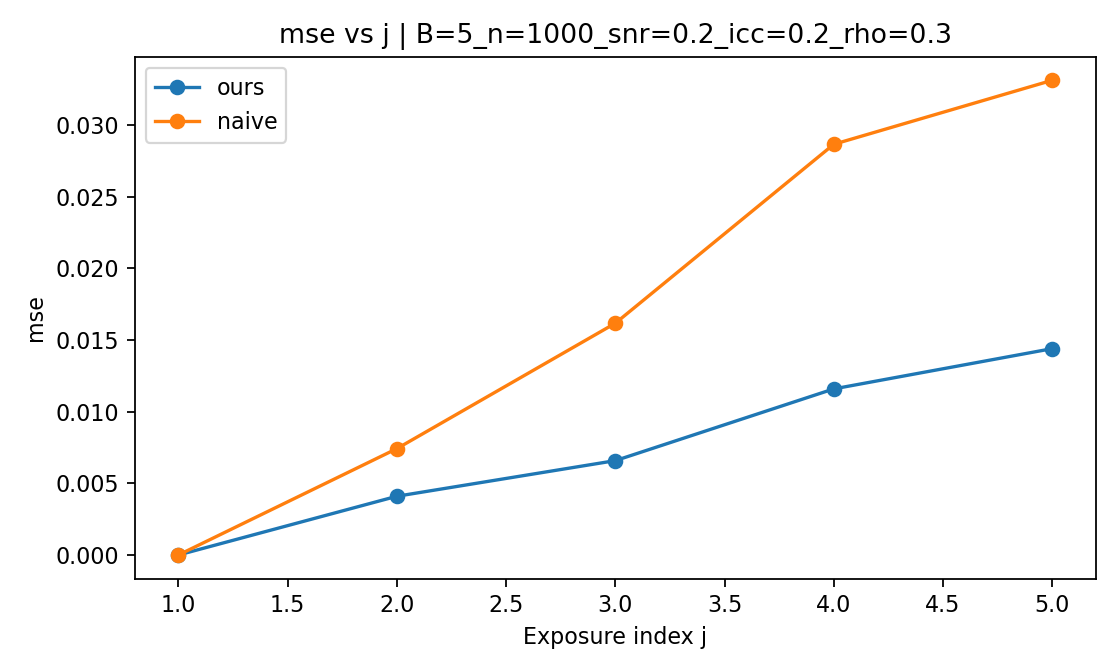
\includegraphics[width=\linewidth]{figures/mse__B=5_n=1000_snr=0.2_icc=0.2_rho=0.3.png}
\end{minipage}
\hfill
\begin{minipage}[b]{0.48\linewidth}
\centering
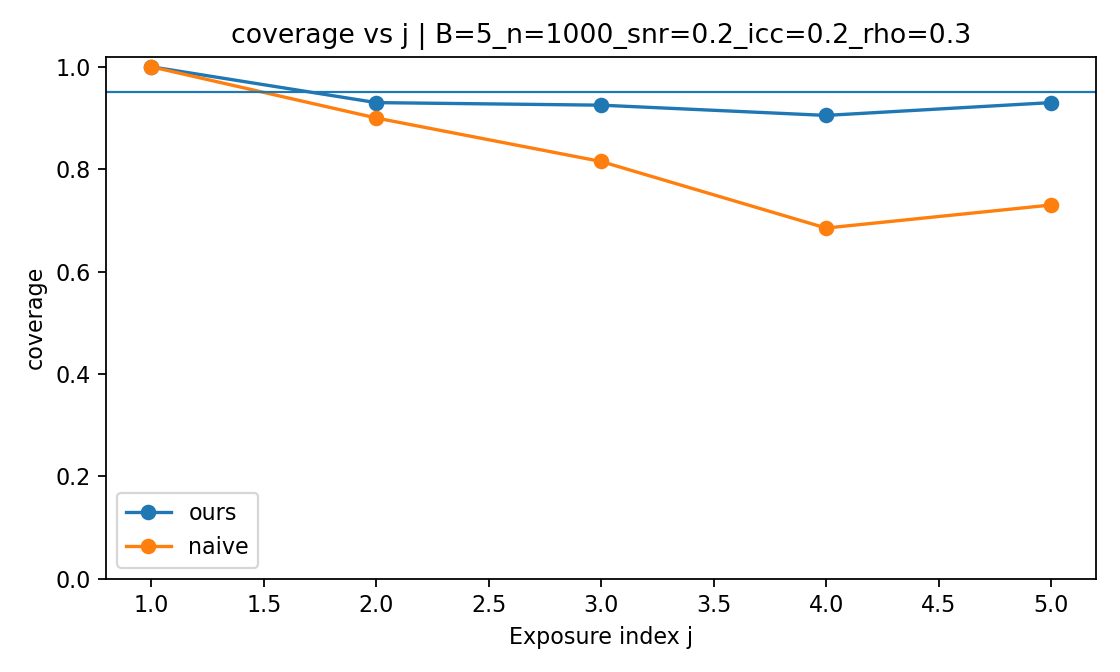
\includegraphics[width=\linewidth]{figures/coverage__B=5_n=1000_snr=0.2_icc=0.2_rho=0.3.png}
\end{minipage}
\Description{Two line plots for a representative scenario with $B=5$ and $n=1000$. The left panel plots mean squared error against the exposure index and shows the proposed estimator below the naive estimator at every exposure. The right panel plots pointwise coverage against the exposure index, with the proposed estimator close to the 95 percent reference line and the naive estimator declining well below nominal coverage at later exposures.}
\caption{Representative finite-sample behavior for $B=5$, $n=1000$, $\mathrm{SNR}=0.2$, $\mathrm{ICC}=0.2$, and $\rho=0.3$. Left: mean squared error by exposure index. Right: pointwise $95\%$ coverage, with the horizontal line marking nominal coverage.}
\label{fig:sim-b5}
\end{figure}

Two features are worth emphasizing. First, the naive estimator can look competitive in standard deviation alone, and in some scenarios it is slightly less variable. Nevertheless, its persistent composition bias dominates the risk comparison, so its MSE remains uniformly larger in our experiments. Second, the difference between the methods is most pronounced when the signal is stronger relative to the noise and when the exposure index is large. This is exactly the regime in which the theoretical distinction between $b_0(j)$ and the naive target is most consequential.

\section{Conclusion}

We study estimation of an exposure-response curve in triangular panel data arising in online experimentation. The proposed additive conditional-mean model yields a simple estimator that adjusts for composition across users with different total exposure counts while retaining a parsimonious representation of the mean surface. Under the model, the estimator is unbiased and asymptotically normal, and the standard user-level bootstrap is valid for inference. In contrast, the naive exposure-wise average generally targets a different limit and can have asymptotically vanishing coverage for the curve of interest.

\bibliographystyle{ACM-Reference-Format}
\bibliography{references}

\end{document}
